\documentclass[12pt,class=report,crop=false]{standalone}
\usepackage[screen]{../python}


\pagestyle{empty}

\begin{document}

% Commande spécifique
\newcommand{\badletter}[1]{\underline{\textcolor{red}{#1}}}



%====================================================================
\chapitre{Visualiseur de texte -- Markdown}
%====================================================================

{\large
La syntaxe \emph{Mardown} est simple, avec un fichier texte bien lisible. Voici quelques éléments de cette syntaxe :
\begin{itemize}
  \item un \textbf{texte en gras} s'obtient en entourant le texte par deux astérisques \ci{**} ;
  \item un \emph{texte en italique} s'obtient en entourant le texte par un astérisque \ci{*} ;
  \item la ligne d'un titre commence par dièse \# ;
  \item la ligne d'un sous-titre commence par deux dièses \#\# ;
  \item pour les éléments d'une liste, chaque ligne commence par un symbole spécial, pour nous ce sera le symbole \og{}plus\fg{} \ci{+}.
\end{itemize}
}

\newpage

\begin{center}
\ci{longueurs =} [8, 11, 9, 14, 8, 8, 15, 10, 14, 11, 15, 15, 5, 12, 9, 9, 15, 10, 14, 5, 12, 8, 8, 13, 10, 11, 8, 13, 7, 5, 6, 11, 7, 7, 13, 6, 6, 9, 8, 12, 5, 8, 7, 6, 6, 15, 13, 11, 7, 12]
\end{center}

\begin{center}
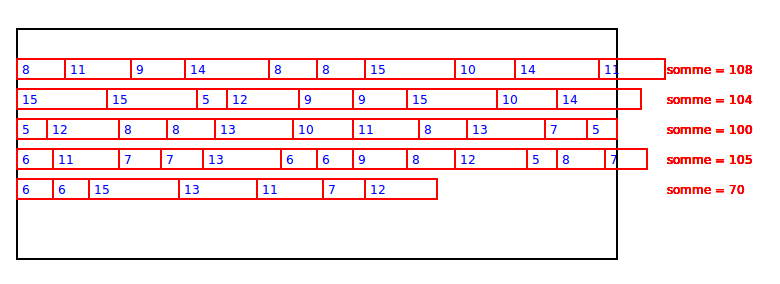
\includegraphics[scale=0.6]{ecran-coupures-1}
\end{center} 


\newpage

  
\begin{center}
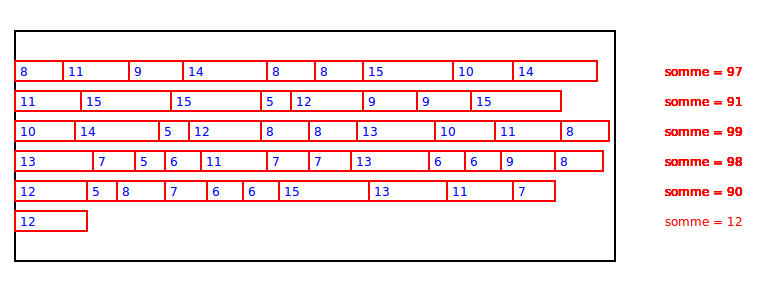
\includegraphics[scale=0.6]{ecran-coupures-2}
\end{center}

\begin{center}
\ci{coupures_simples(longueurs)} 

\bigskip

renvoie \ci{[0, 9, 17, 27, 39, 49, 50]}

\end{center}

\newpage


  
\begin{center}
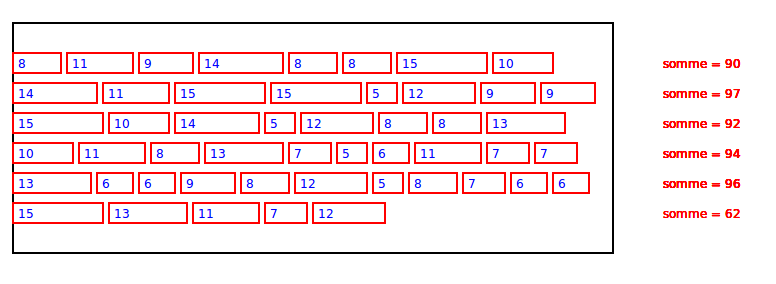
\includegraphics[scale=0.6]{ecran-coupures-3}
\end{center} 

\begin{center}
\ci{coupures_espaces(longueurs)}


\bigskip

renvoie \ci{[0, 8, 16, 24, 34, 45, 50]}
  
  
\end{center}

\newpage


\begin{center}
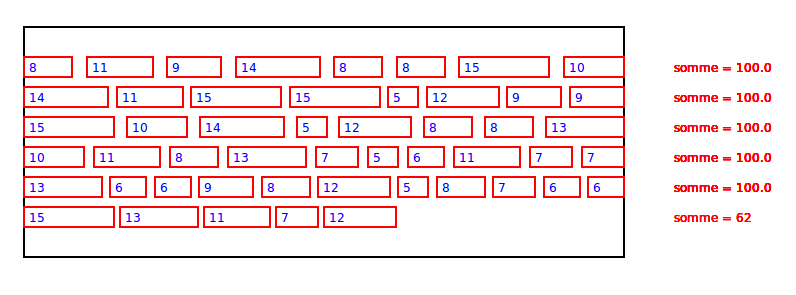
\includegraphics[scale=0.6]{ecran-coupures-4}
\end{center}


\begin{center}
   \ci{calcul_longueur_espaces(longueurs,coupures)} 
   
   \bigskip
   
   \ci{[2.43, 1.43, 2.14, 1.67, 1.40, 1.00]}
\end{center} 
 
\end{document}
